% !TeX spellcheck = en_US
% !TeX program = lualatex

\documentclass[11pt]{beamer}
\usetheme[
    outer/progressbar=foot
    %outer/numbering=none
]{metropolis}
%!TEX root = ../main.tex
%!TEX root = ../main.tex
% Fonts and Encoding
\usepackage{fontspec}

% Graphics
\usepackage{tikz}
\usepackage{pgfplots}
\usepackage{pgfpages}

% Colors
\usepackage{xcolor}
\usepackage{colortbl}

% Math
\usepackage{amsmath}
\usepackage{unicode-math}
\usepackage{stmaryrd}
\usepackage{mathtools}
\usepackage{bussproofs}

% Typesetting
\usepackage{caption}
\usepackage{subcaption}
\usepackage{multirow}
\usepackage{array}
\usepackage{csquotes}

% Layout
\usepackage[a4paper]{geometry}
\usepackage{fancyhdr}
\usepackage{float}

% Code
\usepackage{listings}
\usepackage{algpseudocode}

% Localization
\usepackage[english]{babel}

% References
\usepackage{hyperref}
\usepackage[style=alphabetic,sorting=ynt,backend=biber]{biblatex}


% Other
\usepackage{todonotes}
%!TEX root = ../main.tex
% Colors
\definecolor{ghost-white}{HTML}{F9F8F8}
\definecolor{platinum}{HTML}{E3E2E2}
\definecolor{ash-gray}{HTML}{B6B5B5}
\definecolor{yankees-blue}{HTML}{22223B}
\definecolor{japanese-violet}{HTML}{592B4D}
\definecolor{mountbatten-pink}{HTML}{9F8095}
\definecolor{mountbatten-pink-light}{HTML}{B7A1AE}
\definecolor{deep-ruby}{HTML}{7A3B69}
\definecolor{pewter-blue}{HTML}{8DA1B9}
\definecolor{ming}{HTML}{3A597A}
\definecolor{japanese-indigo}{HTML}{294159}
\definecolor{roman-silver}{HTML}{808D98}
\definecolor{halfgray}{HTML}{7E7E7E}
\definecolor{darkgray}{HTML}{3E3E5E}
\definecolor{solarized-background}{HTML}{FDF6E3}
\definecolor{solarized-background-dark}{HTML}{EEE8D5}
\definecolor{solarized-default}{HTML}{657B83}
\definecolor{solarized-comment}{HTML}{93A1A1}
\definecolor{solarized-green}{HTML}{859900}
\definecolor{solarized-blue}{HTML}{268BD2}
\definecolor{solarized-cyan}{HTML}{2AA198}
%!TEX root = ../main.tex
\setsansfont[Ligatures=TeX]{Calibri}
\setmainfont[Ligatures=TeX]{Times New Roman}
\setmonofont[
	Path = {./Fonts/SourceCodePro/},
	Ligatures = TeX,
	Extension = .otf,
	UprightFont = *-Regular,
	ItalicFont = *-It,
	BoldFont = *-Bold,
	BoldItalicFont = *-BoldIt,
    Scale = MatchLowercase,
    Scale = 0.95
]{SourceCodePro}

\setbeamerfont{alerted text}{series=\bfseries, shape=\scshape, size=\fontsize{12}{16}}
\setbeamerfont{frametitle}{series=\mdseries}
\setbeamerfont{block title alerted}{shape=\upshape, series=\mdseries}
% !TeX root = ../main.tex
% !TeX program = lualatex

\makeatletter
% Literate styling of numbers
\newcommand{\ProcessDigit}[1]
{%
    \ifnum\lst@mode=\lst@Pmode\relax%
    {\ttfamily\color{solarized-cyan} #1}%
    \else
    #1%
    \fi
}

% Local extensions to literate mapping
\def\addToLiterate#1{\edef\lst@literate{\unexpanded\expandafter{\lst@literate}\unexpanded{#1}}}
\lst@Key{add to literate}{}{\addToLiterate{#1}}
\makeatother

\newcommand{\symbolstyle}{\color{solarized-blue}}

\lstset{
    inputencoding       = utf8,
    showspaces          = false,
    showstringspaces    = false,
    numbers             = left,
    belowcaptionskip    = \bigskipamount,
    captionpos          = b,
    frame               = none,
    escapeinside        = {(***}{***)},
    frame               = single,
    rulecolor           = \color{solarized-background-dark},
    framextopmargin     = 1pt,
    framexleftmargin    = 1pt,
    aboveskip           = 1.5em,
    backgroundcolor     = {\color{solarized-background}},
    numberstyle         = {\footnotesize\ttfamily\color{darkgray}},
    emphstyle           = {\color{solarized-blue}},
    commentstyle        = {\it\ttfamily\color{solarized-comment}},
    stringstyle         = {\mdseries\ttfamily\color{solarized-cyan}},
    keywordstyle        = {\bfseries\ttfamily\color{solarized-green}},
    basicstyle          = {\ttfamily\color{solarized-default}},
}

\lstdefinelanguage{agda}{
    morekeywords        = {data,where,module,open,import,using,hiding},
    morekeywords        = {renaming,private,variable,record,with},
    morekeywords        = {constructor,field},
    morecomment         = [l]{--},
    morecomment         = [s]{\{-}{-\}},
    literate            = {bNat}{{\(\mathbb{N}\)}}1
                        {\\bZ}{{\(\mathbb{Z}\)}}1
                        {0}{{{\ProcessDigit{0}}}}1
                        {1}{{{\ProcessDigit{1}}}}1
                        {2}{{{\ProcessDigit{2}}}}1
                        {3}{{{\ProcessDigit{3}}}}1
                        {4}{{{\ProcessDigit{4}}}}1
                        {5}{{{\ProcessDigit{5}}}}1
                        {6}{{{\ProcessDigit{6}}}}1
                        {7}{{{\ProcessDigit{7}}}}1
                        {8}{{{\ProcessDigit{8}}}}1
                        {9}{{{\ProcessDigit{9}}}}1
                        {\ ->\ }{{{\symbolstyle\(\to\)}}}4
                        {:}{{{\symbolstyle{:}}}}1
                        {forall}{{\(\forall\)}}1
                        {\ \\equiv\ }{{{\symbolstyle\(\equiv\)}}}3
                        {\ \\lub\ }{{{\symbolstyle\(\sqcup\)}}}3
                        {\\lub}{{\(\sqcup\)}}1
                        {\\glb}{{\(\sqcap\)}}1
                        {\\lambda}{{{\symbolstyle\(\lambda\)}}}1
                        {-\\leq}{{{\symbolstyle-\(\leq\)}}}2
                        {\ \\leq\ }{{{\symbolstyle\(\leq\)}}}3
                        {\\leq?}{{{\symbolstyle\(\leq\)?}}}2
                        {\\\^r}{{{\(^r\)}}}1
                        {\\\^l}{{{\(^l\)}}}1
                        {\\\_0}{{\(_0\)}}1
                        {\\\_1}{{\(_1\)}}1
                        {\\\_2}{{\(_2\)}}1
                        {\\\_3}{{\(_3\)}}1
                        {\\lceil}{{\(\lceil\)}}1
                        {\\rceil}{{\(\rceil\)}}1
                        {\\lfloor}{{\(\lfloor\)}}1
                        {\\rfloor}{{\(\rfloor\)}}1
                        {\\llog}{{\(\lceil\)log\(_2\)}}5
                        {\\ndiv2ceil}{{\(\lceil\)n/2\(\rceil\)}}5
                        {\\ndiv2floor}{{\(\lfloor\)n/2\(\rfloor\)}}5
                        {=>}{{\(\Rightarrow\)}}1
                        {s\\leqs}{{s\(\leq\)s}}3
                        {z\\leqn}{{z\(\leq\)n}}3
                        {height-\\equiv}{{{\symbolstyle height-\(\equiv\)}}}8
                        {delay-\\leq}{{{\symbolstyle delay-\(\leq\)}}}7
                        {\\equiv}{{\(\equiv\)}}1
                        {\\leq}{{\(\leq\)}}1
                        {\\geq}{{\(\geq\)}}1
                        {\\langle}{{\(\langle\)}}1
                        {\\rangle}{{\(\rangle\)}}1
                        {\\circ}{{\(\circ\)}}1
                        {\\qed}{{\(\qed\)}}1
                        {\\ominus}{{\(\ominus\)}}1
                        {\\nlt}{{\(\not<\)}}1
}
\lstset{language=agda}
%!TEX root = ../main.tex
\graphicspath{ {./Images/} }
\def\arraystretch{1.33}

\pgfplotsset{compat=1.16}

\pagestyle{fancy}

\addbibresource{references.bib}

% ':' with less whitespace
\newcommand{\oftype}{\mathbin{:}}
% abs value symbols as delimiter operator
\DeclarePairedDelimiter\abs{\lvert}{\rvert}

\makeatletter
\newcommand{\ProcessDigit}[1]
{%
    \ifnum\lst@mode=\lst@Pmode\relax%
    {\ttfamily\color{solarized-cyan} #1}%
    \else
    #1%
    \fi
}
\makeatother

\newcommand{\emphstyle}{\bf\color{solarized-blue}}
\lstset{
    inputencoding       = utf8,
    showspaces          = false,
    showstringspaces    = false,
    numbers             = left,
    belowcaptionskip    = \bigskipamount,
    captionpos          = b,
    frame               = none,
    mathescape          = true,
    escapeinside        = {(*}{*)},
    frame               = single,
    rulecolor           = \color{solarized-background-dark},
    framextopmargin     = 1pt,
    framexleftmargin    = 1pt,
    aboveskip           = 1.5em,
    backgroundcolor     = {\color{solarized-background}},
    numberstyle         = {\footnotesize\ttfamily\color{darkgray}},
    emphstyle           = \emphstyle,
    commentstyle        = {\it\ttfamily\color{solarized-comment}},
    stringstyle         = {\mdseries\ttfamily\color{solarized-cyan}},
    keywordstyle        = {\bfseries\ttfamily\color{solarized-green}},
    basicstyle          = {\ttfamily\color{solarized-default}},
}

\lstdefinelanguage{agda}{
    morekeywords        = {data,where,module,open,import,using,hiding},
    morekeywords        = {renaming,private,variable,record,with},
    emph                = {:,->},
    morecomment         = [l]{--},
    morecomment         = [s]{\{-}{-\}},
    literate            = {bNat}{{\(\mathbb{N}\)}}1
                        {0}{{{\ProcessDigit{0}}}}1
                        {1}{{{\ProcessDigit{1}}}}1
                        {2}{{{\ProcessDigit{2}}}}1
                        {3}{{{\ProcessDigit{3}}}}1
                        {4}{{{\ProcessDigit{4}}}}1
                        {5}{{{\ProcessDigit{5}}}}1
                        {6}{{{\ProcessDigit{6}}}}1
                        {7}{{{\ProcessDigit{7}}}}1
                        {8}{{{\ProcessDigit{8}}}}1
                        {9}{{{\ProcessDigit{9}}}}1
                        {<=}{{\(\leq\)}}1
                        {->}{{{\emphstyle\(\to\)}}}1
                        {:}{{{\emphstyle{:}}}}1
                        {forall}{{\(\forall\)}}1
                        {\\equiv}{{\(\equiv\)}}1,
}
\lstset{language=agda}

% For todonotes
\setlength{\marginparwidth}{3cm}


\title{Modelling Resource Constraints in a Dependently Typed Language}
\author{Lia Schütze}

\begin{document}
    \maketitle
    \begin{frame}{In defense of types}
        Types: Very useful to encode guarantees to be checked by the compiler

        \begin{itemize}
            \item[\usebeamertemplate{itemize item}] Avoid mixing of data
            \item[\usebeamertemplate{itemize item}] Memory safety
            \item[\usebeamertemplate{itemize item}] Programmer-specified constraints
            \item[\usebeamertemplate{itemize item}] And more!
        \end{itemize}

        Can we use it to guarantee runtime bounds?
    \end{frame}

    \begin{frame}{In this thesis}
        \begin{itemize}
            \item[\usebeamertemplate{itemize item}] Deterministic worst-case bounds
            \item[\usebeamertemplate{itemize item}] Amortized worst-case bounds
        \end{itemize}
    \end{frame}

    \section{Deterministic Worst-Case Bounds}

    \begin{frame}{Measuring runtime}
        \begin{itemize}
            \item[\usebeamertemplate{itemize item}] Wall-clock time % - can't be determined at compile time
            \item[\usebeamertemplate{itemize item}] Instructions % - possible, but we are far from the metal
            \item[\usebeamertemplate{itemize item}] User-defined measure % circumventable
            \item[\usebeamertemplate{itemize item}] Comparisons or similar metrics
        \end{itemize}
    \end{frame}

    \begin{frame}{Wall-clock time}
        On input of size $x$, executes in $f(x)$ nanoseconds.

        \begin{itemize}[leftmargin=3em]
            \item[\textbf{Pro}] Most accurate measure
            \item[\textbf{Con}] Impossible to determine at compile time
        \end{itemize}
    \end{frame}

    \begin{frame}{Instructions}
        On input of size $x$, executes in $f(x)$ instructions.

        \begin{itemize}[leftmargin=3em]
            \item[\textbf{Pro}] Still pretty accurate
            \item[\textbf{Con}] Harder the further we are from the metal
        \end{itemize}
    \end{frame}

    \begin{frame}[fragile]{User-defined measure}
        On input of size $x$, executes $f(x)$ ``ticks"

        \begin{lstlisting}[emph={Thunk,tick, return}]
Thunk : Set -> bNat -> Set
Thunk A n = A

return : A -> Thunk A 0
return a = a

tick : A -> Thunk A 1
tick a = a

_>>=_ :  Thunk A n -> (A -> Thunk B m) -> Thunk B (n + m)
x >>= f = f x
        \end{lstlisting}
    \end{frame}

    \begin{frame}{User-defined measure}
        \begin{itemize}[leftmargin=3em]
            \item[\textbf{Pro}] Flexible
            \item[\textbf{Con}] Relies on programmer to manage time correctly
        \end{itemize}
    \end{frame}

    \begin{frame}{Comparisons as metric}
        On input of size $x$, executes $f(x)$ comparisons

        \begin{itemize}[leftmargin=3em]
            \item[\textbf{Pro}] Familiar metric from algorithm analysis
            \item[\textbf{Con}] Limited applicability
        \end{itemize}
    \end{frame}

    \begin{frame}[fragile]
        Hide information from programmer:

        \begin{lstlisting}[emph=compare]
compare : A -> A -> Bool
compare x y = ?
        \end{lstlisting}

        $\Rightarrow$ Programmer can't perform comparisons without us
    \end{frame}

    \begin{frame}{The Framework}
        Model computation as a decision tree:

        \vskip 2em

        \begin{center}
            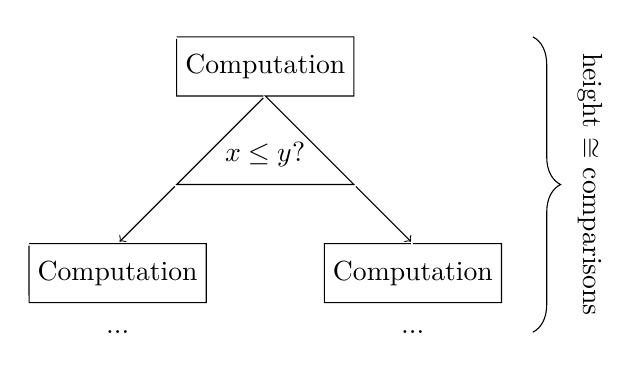
\begin{tikzpicture}[scale=0.75]
\usetikzlibrary{decorations.pathreplacing}

% \node [shape = rectangle, draw = black, minimum size = 2em] at (0,2) {Computation};
\node at (0,2) {Computation};
\node at (0,0.5) {$x \le y?$};
\node (v2) at (-2.5,-1.5) {Computation};
\node (v4) at (2.5,-1.5) {Computation};
% \draw (-1,.15) node (v1) {}  -- (0,1.65) -- (1,.15) node (v3) {} -- cycle;
\node at (-2.5,-2.5) {$\ldots$};
\node at (2.5,-2.5) {$\ldots$};
\draw [decorate,decoration={brace,mirror,amplitude=10,raise=-10}] (5,-2.5) -- (5,2.5) node {};
\node [rotate=-90] at (5.5,0) {height $\cong$ comparisons};
\draw (-1.5,2.5) node [inner sep=0] (v6) {} -- (1.5,2.5) node [inner sep = 0] (v9) {} -- (1.5,1.5) -- (0,1.5) node [inner sep=0] (v5) {} -- (1.5,0) node [inner sep=0] (cornerR) {} -- (-1.5,0) node [inner sep=0] (cornerL) {} -- (v5) -- (-1.5,1.5) -- (v6);
\draw (-4,-1) node [inner sep = 0] (v1) {} -- (-2.5,-1) node [inner sep=0] (v2) {} -- (-1,-1) -- (-1,-2) -- (-4,-2) -- (v1);

\draw (2.5,-1) node [inner sep=0] (v3) {} -- (4,-1) -- (4,-2) -- (1,-2) -- (1,-1) -- (v3);
\draw [->] (cornerL) edge (v2);
\draw [->] (cornerR) edge (v3);
\end{tikzpicture}
        \end{center}
    \end{frame}

    \begin{frame}[fragile]{The Framework}
        Model computation as a decision tree:

        \begin{lstlisting}[emph={DecTree}]
data DecTree (C : Set) (A : Set) : (d : bNat) -> Set where
    ...
        \end{lstlisting}

        \uncover<2->{
        Parameterized by:

        \begin{itemize}
            \item[\texttt{C}:]<2-> Comparison type
            \item[\texttt{A}:]<3-> Return type
            \item[\texttt{d}:]<4> Depth of the tree \quad $\cong$ \quad \#Comparisons
        \end{itemize}
        }
    \end{frame}

    \begin{frame}[fragile]{The Framework - Constructors}
        \begin{lstlisting}[emph={DecTree,return}]
data DecTree (C : Set) (A : Set) : (d : bNat) -> Set where
    ...
    return : A -> DecTree C A 0
    ...
        \end{lstlisting}
    \end{frame}

    \begin{frame}[fragile]{The Framework - Constructors}
        \begin{lstlisting}[emph={DecTree}]
data DecTree (C : Set) (A : Set) : (d : bNat) -> Set where
    ...
    _>>=_ :  DecTree C A' h\_1
          -> (A' -> DecTree C A h\_2)
          -> DecTree C A (h\_1 + h\_2)
    ...
        \end{lstlisting}
    \end{frame}

    \begin{frame}[fragile]{The Framework - Constructors}
        \begin{lstlisting}[emph={DecTree,delay}]
data DecTree (C : Set) (A : Set) : (d : bNat) -> Set where
    ...
    delay : (d : bNat) -> DecTree C A h -> DecTree C A (h + d)
        \end{lstlisting}
    \end{frame}

    \begin{frame}[fragile]{The Framework - Constructors}
        \begin{lstlisting}[emph={DecTree}]
data DecTree (C : Set) (A : Set) : (d : bNat) -> Set where
    ...
    if_\leq?_then_else_ :  (x y : C)
                     -> DecTree C A h\_1
                     -> DecTree C A h\_2
                     -> DecTree C A (suc (h\_1 \lub h\_2))
    ...
        \end{lstlisting}
    \end{frame}

    \begin{frame}[fragile]{A Simple Example}
        \begin{lstlisting}[emph={min,if,then,else,return}]
min : A -> A -> DecTree A A 1
min x y = if x !leq y
          then return x
          else return y
        \end{lstlisting}
    \end{frame}

    \begin{frame}[fragile]{Evaluating Computations}
        \begin{lstlisting}[emph={reduce}]
reduce :  (\leq : C -> C -> Bool)
       -> DecTree C A h
       -> A
reduce _?leq_ (return val) = val
reduce _?leq_ (comp >>= f) = reduce _?leq_ (f $ reduce _?leq_ comp)
reduce _?leq_ (delay comp) = reduce _?leq_ comp
reduce _?leq_ (if x !leq y then left else right) with x ?leq y
... | true  = reduce _?leq_ left
... | false = reduce _?leq_ right
        \end{lstlisting}
    \end{frame}

    \begin{frame}[fragile]{In Action - Mergesort}
        \begin{lstlisting}[emph={merge,sort,bound,split,return},showlines=true]
merge-sort : Vec A l -> DecTree A (Vec A l) (l * \lceillog\_2 l \rceil)











        \end{lstlisting}
    \end{frame}

    \begin{frame}[fragile]{In Action - Mergesort}
        \begin{lstlisting}[emph={merge,sort,bound,split,return},showlines=true]
merge-sort : Vec A l -> DecTree A (Vec A l) (l * \lceillog\_2 l \rceil)
merge-sort [] = return []










        \end{lstlisting}
    \end{frame}

    \begin{frame}[fragile]{In Action - Mergesort}
        \begin{lstlisting}[emph={merge,sort,bound,split,return},showlines=true]
merge-sort : Vec A l -> DecTree A (Vec A l) (l * \lceillog\_2 l \rceil)

merge-sort (x :: []) = return (x :: [])









        \end{lstlisting}
    \end{frame}

    \begin{frame}[fragile]{In Action - Mergesort}
        \begin{lstlisting}[emph={merge,sort,bound,split,return},showlines=true]
merge-sort : Vec A l -> DecTree A (Vec A l) (l * \lceillog\_2 l \rceil)


merge-sort xs@(_ :: _ :: _) =
                                      do
        let (left , right) = split xs






        \end{lstlisting}
    \end{frame}

    \begin{frame}[fragile]{In Action - Mergesort}
        \begin{lstlisting}[emph={merge,sort,bound,split,return},showlines=true]
merge-sort : Vec A l -> DecTree A (Vec A l) (l * \lceillog\_2 l \rceil)


merge-sort xs@(_ :: _ :: _) =
                                      do
        let (left , right) = split xs
        res-left <- merge-sort left
        -- \lceil l /2\rceil * \lceillog\_2 \lceil l /2\rceil \rceil
        res-right <- merge-sort right
        -- \lfloor l /2\rfloor * \lceillog\_2 \lfloor l /2\rfloor \rceil


        \end{lstlisting}
    \end{frame}

    \begin{frame}[fragile]{In Action - Mergesort}
        \begin{lstlisting}[emph={merge,sort,bound,split,return},showlines=true]
merge-sort : Vec A l -> DecTree A (Vec A l) (l * \lceillog\_2 l \rceil)


merge-sort xs@(_ :: _ :: _) =
                                      do
        let (left , right) = split xs
        res-left <- merge-sort left
        -- \lceil l /2\rceil * \lceillog\_2 \lceil l /2\rceil \rceil
        res-right <- merge-sort right
        -- \lfloor l /2\rfloor * \lceillog\_2 \lfloor l /2\rfloor \rceil
        merge res-left res-right
        -- \lceil l /2\rceil + \lfloor l /2\rfloor
        \end{lstlisting}
    \end{frame}

    \begin{frame}[fragile]{In Action - Mergesort}
        \begin{lstlisting}[emph={merge,sort,bound,split,return},showlines=true]
merge-sort : Vec A l -> DecTree A (Vec A l) (l * \lceillog\_2 l \rceil)


merge-sort xs@(_ :: _ :: _) =
    delay-\leq (merge-sort-bound _) $ do
        let (left , right) = split xs
        res-left <- merge-sort left
        -- \lceil l /2\rceil * \lceillog\_2 \lceil l /2\rceil \rceil
        res-right <- merge-sort right
        -- \lfloor l /2\rfloor * \lceillog\_2 \lfloor l /2\rfloor \rceil
        merge res-left res-right
        -- \lceil l /2\rceil + \lfloor l /2\rfloor
        \end{lstlisting}
    \end{frame}

    \section{Amortized Bounds}

    \begin{frame}{Amortized Runtime}
        Consider aggregate sequences of operations:

        \begin{tabular}{rlr}
          & One operation in & $\mathcal O(n)$ \\
        + & $n-1$ operations in & $\mathcal O(1)$ \\
        = & $n$ operations in & $\mathcal O(n)$
        \end{tabular}

        \vskip 2em

        $\Rightarrow$ On average, operations take time $\mathcal O(1)$.
    \end{frame}

    \begin{frame}{Potential Method}
        Objects $v$ have potential $\varphi(v)$ such that

        \begin{itemize}
            \item $\varphi(v) \geq 0$
            \item $\varphi(v_0) = 0$
        \end{itemize}
    \end{frame}

    \begin{frame}{Potential Method}
        Operations $o$ taking object $v$ to $v'$ have amortized runtime $t_a(o) = t(o) - \varphi(v) + \varphi(v')$.

        Aggregate runtime: $\sum t_a(o) = (\sum t(o)) - \varphi(v_0) + \varphi(v_n)$
    \end{frame}

    \begin{frame}[fragile]{Defining Potential in Code}
        \begin{lstlisting}[emph={Amortized}]
record Amortized {I : Set} (A : I -> Set) : Set where
    field
        {i\_0} : I
        initial : A i\_0
        potential : A i -> bNat
        init\equiv0 : potential initial \equiv 0
        \end{lstlisting}
    \end{frame}

    \begin{frame}{Amortized Computations}
        Model an amortized computation as

        \begin{itemize}
            \item A record of the last value
            \item A deterministic computation on that value
        \end{itemize}
    \end{frame}

    \begin{frame}[fragile]{Amortized Computation}
        \begin{lstlisting}[emph={Am,Amortized}]
data Am {I : Set} {A : I -> Set}
        (am : Amortized A)
        (C : Set)
          : Set where
    ...
        \end{lstlisting}
    \end{frame}

    \begin{frame}[fragile]{Amortized Computation - Base}
        \begin{lstlisting}[emph={Am,base}]
data Am ... where
    base :  (x : A (Amortized.i\_0 am))
         -> {x \equiv Amortized.initial am}
         -> Am am C
        \end{lstlisting}
    \end{frame}

    \begin{frame}[fragile]{Amortized Computation - Step}
        \begin{lstlisting}[emph={Am,step}]
data Am ... where
    step :  {next : A i -> I}
            {time : A i -> bNat}
         -> Am am C
         -> ((x : A i) -> DecTree C (A $ next x) (time x))
         -> Am am C
        \end{lstlisting}
    \end{frame}

    \begin{frame}[fragile]{Amortized Computation - Determining Runtime}
        \begin{lstlisting}[emph={atime,step,base}]
atime-step : {am : Amortized A} -> Am am C -> \bZ
atime-step (base _) = 0
atime-step (step {_} {time} val f) =
        dtime - pot-before + pot-after
    where
        dtime      = time (eval val)
        pot-before = potential (eval val)
        pot-after  = potential (reduce $ f $ eval val)
        \end{lstlisting}
    \end{frame}

    \begin{frame}[fragile]{Amortized Computation - Determining Runtime}
        \begin{lstlisting}[emph={atime,full}]
atime-full : {am : Amortized A} -> Am am C -> \bZ
atime-full (base _) = 0
atime-full v@(step val f) = atime-full val + atime-step v
        \end{lstlisting}
    \end{frame}

    \begin{frame}{Binomial Heaps}
        Data structure with amortized $\mathcal O(1)$ insertion.

        Heap is collection of binomial trees.
    \end{frame}

    \begin{frame}{Binomial Trees}
        Organized by \emph{rank}.

        Rank $n$ tree has $2^n$ nodes.
    \end{frame}

    \begin{frame}{Binomial Tree}
        Rank $0$: Single node

        \vskip 2em

        \begin{center}
        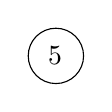
\begin{tikzpicture}

\node [shape = circle, minimum size = 2em, draw=black] at (0,0) {$5$};
\end{tikzpicture}
        \end{center}
    \end{frame}

    \begin{frame}{Binomial Tree}
        Rank $1$: Node with rank $0$ child

        \vskip 2em

        \begin{center}
            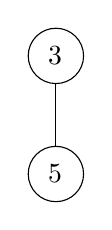
\begin{tikzpicture}

\node [shape=circle, minimum size = 2em, draw=black] (v1) at (0,0) {$3$};
\node [shape=circle, minimum size = 2em, draw=black] (v2) at (0,-1.5) {$5$};
\draw  (v1) edge (v2);
\end{tikzpicture}
        \end{center}
    \end{frame}

    \begin{frame}{Binomial Tree}
        Rank $2$: Node with rank $1$ and rank $2$ child

        \vskip 2em

        \begin{center}
            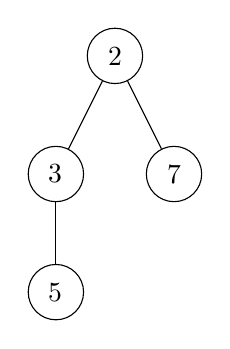
\begin{tikzpicture}
\node [shape=circle, minimum size = 2em, draw=black] (v3) at (3.75,0) {$2$};
\node [shape=circle, minimum size = 2em, draw=black] (v6) at (4.5,-1.5) {$7$};
\node [shape=circle, minimum size = 2em, draw=black] (v4) at (3,-1.5) {$3$};
\node [shape=circle, minimum size = 2em, draw=black] (v5) at (3,-3) {$5$};
\draw  (v3) edge (v4);
\draw  (v4) edge (v5);
\draw  (v3) edge (v6);
\end{tikzpicture}
        \end{center}
    \end{frame}

    \begin{frame}{Binomial Heaps}
        Example: Binomial heap with $6 = 2^1 + 2^2$ entries

        \begin{center}
            \begin{tikzpicture}
\node [draw = black, minimum size = 2em] (list0) at (2em,0.5em) {};
\node [draw = black, cross out, minimum size = 2em] at (2em,0.5em) {};
\node [draw = black, minimum size = 2em] (list1) at (4em,0.5em) {};
\node [draw = black, minimum size = 2em] (list2) at (6em,0.5em) {};


\node [draw = black, shape = circle, minimum size = 2em] (v1) at (0em,-1.5) {$3$};
\node [draw = black, shape = circle, minimum size = 2em] (v2) at (0em,-3) {$5$};
\draw  (v1) edge (v2);
\path [draw, -latex'] (list1.south) -- ++(0,-.75em) node(bar) {} -| (v1);


\node [draw = black, shape = circle, minimum size = 2em] (v3) at (8em,-1.5) {$2$};
\node [draw = black, shape = circle, minimum size = 2em] (v4) at (6em,-3) {$3$};
\node [draw = black, shape = circle, minimum size = 2em] (v6) at (10em,-3) {$7$};
\node [draw = black, shape = circle, minimum size = 2em] (v5) at (6em,-4.5) {$5$};
\draw  (v3) edge (v4);
\draw  (v4) edge (v5);
\draw  (v3) edge (v6);
\path [draw, -latex'] (list2.south) -- ++(0,-.75em) node(foo) {} -| (v3);
\end{tikzpicture}
        \end{center}
    \end{frame}

    \begin{frame}[fragile]{Binomial Trees - Implementation}
        \begin{lstlisting}[emph={DescList,BinTree,base,cons,Leaf,Node}]
data DescList (A : bNat -> Set) : bNat -> Set where
    base : A 0 -> DescList 0
    cons : A (suc l) -> DescList A l -> DescList A (suc l)

data BinTree (A : Set) : (rank : bNat) -> Set where
    Leaf : A -> BinTree 0
    Node : A -> DescList (BinTree A) l -> BinTree A (suc l)
        \end{lstlisting}
    \end{frame}

    \begin{frame}[fragile]{Binomial Heaps - Implementation}
        \begin{lstlisting}[add to literate={{::}{{{::}}}2},emph={BinHeap,nil,empty,entry}]
data BinHeap (A : Set) : (rnk : bNat) -> (sze : bNat) -> Set where
    nil       : BinHeap A l 0
    empty::   : BinHeap A (suc l) n -> BinHeap A l n
    entry_::_ :  BinTree A l
              -> BinHeap A (suc l) n
              -> BinHeap A l (2 ^ l + n)
        \end{lstlisting}
    \end{frame}

    \begin{frame}[fragile]{Amortized Computation}
        \begin{lstlisting}[emph={BinHeap,heap,amortized}]
heap-amortized : (A : Set) -> Amortized (BinHeap A 0)
Amortized.i\_0        (heap-amortized A) = 0
Amortized.initial   (heap-amortized A) = nil
Amortized.potential (heap-amortized A) = entries
Amortized.init\equiv0    (heap-amortized A) = refl
        \end{lstlisting}
    \end{frame}

    \begin{frame}{Inserting into Heaps}
        \begin{center}
            \begin{tikzpicture}
\node [draw = black, minimum size = 2em] (list0) at (0em, 0em) {};
\node [draw = black, minimum size = 2em] (list1) at (2em, 0em) {};
\node [draw = black, minimum size = 2em] (list2) at (4em, 0em) {};
\node [draw = black, minimum size = 2em, cross out] at (4em, 0em) {};
\node [draw = black, minimum size = 2em] (list3) at (6em, 0em) {};

\node [draw = black, shape = circle, minimum size = 1.5em] (t00) at (0em, -5em) {$3$};
\path [draw, -latex'] (list0.south) -- (t00);

\node [draw = black, shape = circle, minimum size = 1.5em] (t10) at (2em, -5em) {$7$};
\node [draw = black, shape = circle, minimum size = 1.5em] (t11) at (2em, -8em) {$9$};
\path [draw, -latex'] (list1.south) -- (t10);
\path [draw] (t10) -- (t11);

\node [shape = circle, minimum size = 1.5em] (t3) at (6em, -5em) {$\ldots$};
\path [draw, -latex'] (list3.south) -- (t3);

\node [draw = black, shape = circle, minimum size = 1.5em] (ins) at (-4em, -5em) {$5$};
\path [draw, dashed, -latex'] (ins) -- ++(0em, 7em) -- ++(4em, 0em) -| (list0.north);
\end{tikzpicture}
        \end{center}
    \end{frame}

    \begin{frame}{Inserting into Heaps}
        \begin{center}
            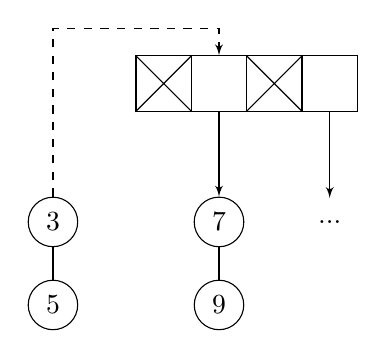
\begin{tikzpicture}
\usetikzlibrary{shapes.misc, arrows}

\node [draw = black, minimum size = 2em] (list0) at (0em, 0em) {};
\node [draw = black, minimum size = 2em, cross out] at (0em, 0em) {};
\node [draw = black, minimum size = 2em] (list1) at (2em, 0em) {};
\node [draw = black, minimum size = 2em] (list2) at (4em, 0em) {};
\node [draw = black, minimum size = 2em, cross out] at (4em, 0em) {};
\node [draw = black, minimum size = 2em] (list3) at (6em, 0em) {};


\node [draw = black, shape = circle, minimum size = 1.5em] (t10) at (2em, -5em) {$7$};
\node [draw = black, shape = circle, minimum size = 1.5em] (t11) at (2em, -8em) {$9$};
\path [draw, -latex'] (list1.south) -- (t10);
\path [draw] (t10) -- (t11);

\node [shape = circle, minimum size = 1.5em] (t3) at (6em, -5em) {$\ldots$};
\path [draw, -latex'] (list3.south) -- (t3);

\node [draw = black, shape = circle, minimum size = 1.5em] (ins0) at (-4em, -5em) {$3$};
\node [draw = black, shape = circle, minimum size = 1.5em] (ins1) at (-4em, -8em) {$5$};
\path [draw] (ins0) -- (ins1);

\path [draw, dashed, -latex'] (ins0) -- ++(0em, 7em) -| (list1.north);
\end{tikzpicture}
        \end{center}
    \end{frame}

    \begin{frame}{Inserting into Heaps}
        \begin{center}
            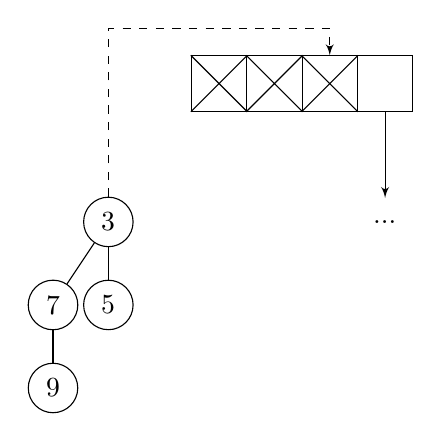
\begin{tikzpicture}
\usetikzlibrary{shapes.misc, arrows}

\node [draw = black, minimum size = 2em] (list0) at (0em, 0em) {};
\node [draw = black, minimum size = 2em, cross out] at (0em, 0em) {};
\node [draw = black, minimum size = 2em] (list1) at (2em, 0em) {};
\node [draw = black, minimum size = 2em, cross out] at (2em, 0em) {};
\node [draw = black, minimum size = 2em] (list2) at (4em, 0em) {};
\node [draw = black, minimum size = 2em, cross out] at (4em, 0em) {};
\node [draw = black, minimum size = 2em] (list3) at (6em, 0em) {};



\node [shape = circle, minimum size = 1.5em] (t3) at (6em, -5em) {$\ldots$};
\path [draw, -latex'] (list3.south) -- (t3);

\node [draw = black, shape = circle, minimum size = 1.5em] (ins0) at (-4em, -5em) {$3$};
\node [draw = black, shape = circle, minimum size = 1.5em] (ins1) at (-4em, -8em) {$5$};
\path [draw] (ins0) -- (ins1);

\node [draw = black, shape = circle, minimum size = 1.5em] (ins2) at (-6em, -8em) {$7$};
\node [draw = black, shape = circle, minimum size = 1.5em] (ins3) at (-6em, -11em) {$9$};
\path [draw] (ins0) -- (ins2);
\path [draw] (ins2) -- (ins3);


\path [draw, dashed, -latex'] (ins0) -- ++(0em, 7em) -| (list2.north);
\end{tikzpicture}
        \end{center}
    \end{frame}

    \begin{frame}{Inserting into Heaps}
        \begin{center}
            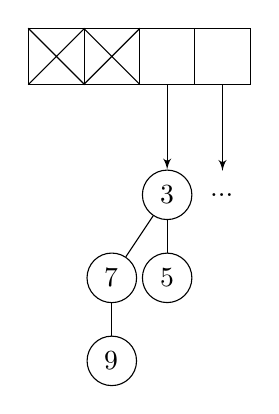
\begin{tikzpicture}
\usetikzlibrary{shapes.misc, arrows}

\node [draw = black, minimum size = 2em] (list0) at (0em, 0em) {};
\node [draw = black, minimum size = 2em, cross out] at (0em, 0em) {};
\node [draw = black, minimum size = 2em] (list1) at (2em, 0em) {};
\node [draw = black, minimum size = 2em, cross out] at (2em, 0em) {};
\node [draw = black, minimum size = 2em] (list2) at (4em, 0em) {};
\node [draw = black, minimum size = 2em] (list3) at (6em, 0em) {};



\node [shape = circle, minimum size = 1.5em] (t3) at (6em, -5em) {$\ldots$};
\path [draw, -latex'] (list3.south) -- (t3);

\node [draw = black, shape = circle, minimum size = 1.5em] (ins0) at (4em, -5em) {$3$};
\node [draw = black, shape = circle, minimum size = 1.5em] (ins1) at (4em, -8em) {$5$};
\path [draw] (ins0) -- (ins1);

\node [draw = black, shape = circle, minimum size = 1.5em] (ins2) at (2em, -8em) {$7$};
\node [draw = black, shape = circle, minimum size = 1.5em] (ins3) at (2em, -11em) {$9$};
\path [draw] (ins0) -- (ins2);
\path [draw] (ins2) -- (ins3);

\path [draw, -latex'] (list2.south) -- (ins0);

\end{tikzpicture}
        \end{center}

        In $\mathcal O(\log n)$ in the worst case, but $\mathcal O(1)$ amortized!
    \end{frame}

    \begin{frame}[fragile]{Inserting into Heaps}
        \begin{lstlisting}[emph={BinTree,BinHeap,entry,empty,nil}]
insert :  BinTree A r
       -> (h : BinHeap A r n)
       -> DecTree A (BinHeap A r (2 ^ r + n))
               (leadingEntries h)
insert t nil = return $ entry t :: nil
insert t (empty:: ts) = return $ entry t :: ts
insert t (entry t' :: ts) = do
    t-join <- link t t'
    empty:: <$> insert t-join ts
        \end{lstlisting}
    \end{frame}

    \begin{frame}[fragile]{Defining an Amortized Computation}
        \begin{lstlisting}[emph={n,inserts}]
n-inserts : Vec A n -> Am (heap-amortized A) A
n-inserts [] = base nil {refl}
n-inserts (x :: xs) = step (n-inserts xs)
                           (\lambda ts -> insert (Leaf x) ts)
        \end{lstlisting}
    \end{frame}

    \begin{frame}[fragile]{Showing Amortized Bounds}
        \begin{lstlisting}[emph={insert,invariant}]
insert-invariant :  (t : BinTree A r)
                 -> (ts : BinHeap A r n)
                 ->   leadingEntries ts
                      - entries ts
                      + entries (reduce $ insert t ts)
                    \equiv 1
        \end{lstlisting}
    \end{frame}

    \begin{frame}[fragile]{Showing Amortized Bounds}
        \begin{lstlisting}[emph={insert,invariant}]
-- 0 - 0 + 1 = 1
insert-invariant t nil = refl
        \end{lstlisting}
    \end{frame}

    \begin{frame}[fragile]{Showing Amortized Bounds}
        \begin{lstlisting}[emph={insert,invariant}]
-- 0 - a + (suc a) = 1
insert-invariant t (empty:: ts) = 0-a+suc[a]\equiv1 (entries ts)
        \end{lstlisting}
    \end{frame}

    \begin{frame}[fragile]{Showing Amortized Bounds}
        \begin{lstlisting}[emph={insert,invariant}]
insert-invariant t ts@(entry x :: ts') = begin
    leadingEntries ts
    - entries ts
    + entries (reduce $ insert t ts)

        \equiv\langle {- reduction -} \rangle

    leadingEntries ts'
    - entries ts'
    + entries (reduce $ insert t ts)

        \equiv\langle ... \rangle
    ...
        \end{lstlisting}
    \end{frame}

    \begin{frame}[fragile]{Showing Amortized Bounds}
        \begin{lstlisting}[emph={insert,invariant}]
insert-invariant t ts@(entry x :: ts') = begin
    ...
        \equiv\langle ... \rangle

    leadingEntries ts'
    - entries ts'
    + entries (reduce $ insert t ts)

        \equiv\langle {- reduction -} \rangle

    leadingEntries ts'
    - entries ts'
    + entries (reduce $ insert (reduce $ link t x) ts')

        \equiv\langle ... \rangle
    ...
        \end{lstlisting}
    \end{frame}

    \begin{frame}[fragile]{Showing Amortized Bounds}
        \begin{lstlisting}[emph={insert,invariant}]
insert-invariant t ts@(entry x :: ts') = begin
    ...
        \equiv\langle ... \rangle

    leadingEntries ts'
    - entries ts'
    + entries (reduce $ insert (reduce $ link t x) ts')

        \equiv\langle {- induction on (link t x), ts -} \rangle

    1   \qed
        \end{lstlisting}
    \end{frame}

    \begin{frame}[fragile]{Showing Amortized Bounds}
        \begin{lstlisting}[emph={insert,in,linear,time}]
insert-in-linear-time :  (xs : Vec A n)
                      -> atime-full (n-inserts xs) \equiv n
insert-in-linear-time [] = refl
        \end{lstlisting}
    \end{frame}

    \begin{frame}[fragile]{Showing Amortized Bounds}
        \begin{lstlisting}[emph={insert,in,linear,time}]
insert-in-linear-time :  (xs : Vec A n)
                      -> atime-full (n-inserts xs) \equiv n
insert-in-linear-time xss@(x :: xs) = begin
    atime-full (n-inserts xss)

         \equiv\langle {- reduction -} \rangle

    atime-full (n-inserts xs)
    + (leadingEntries (am-eval $ n-inserts xs)
       - am-potential (n-inserts xs)
       + am-potential (n-inserts xss))

        \equiv\langle ... \rangle
    ...
        \end{lstlisting}
    \end{frame}

    \begin{frame}[fragile]{Showing Amortized Bounds}
        \begin{lstlisting}[emph={insert,in,linear,time}]
insert-in-linear-time :  (xs : Vec A n)
                      -> atime-full (n-inserts xs) \equiv n
insert-in-linear-time xss@(x :: xs) = begin
    ...
        \equiv\langle ... \rangle

    atime-full (n-inserts xs)
    + (leadingEntries (am-eval $ n-inserts xs)
       - am-potential (n-inserts xs)
       + am-potential (n-inserts xss))

        \equiv\langle {- insert invariant -} \rangle

    atime-full (n-inserts xs) + 1

        \equiv\langle ... \rangle
    ...
        \end{lstlisting}
    \end{frame}

    \begin{frame}[fragile]{Showing Amortized Bounds}
        \begin{lstlisting}[emph={insert,in,linear,time}]
insert-in-linear-time :  (xs : Vec A n)
                      -> atime-full (n-inserts xs) \equiv n
insert-in-linear-time xss@(x :: xs) = begin
    ...
        \equiv\langle ... \rangle

    atime-full (n-inserts xs) + 1

        \equiv\langle {- induction on xs -} \rangle

    (n - 1) + 1

        \equiv\langle\rangle

    n   \qed
        \end{lstlisting}
    \end{frame}

\section{Summary}
    \begin{frame}{Summary}
        \begin{itemize}
            \item[\usebeamertemplate{itemize item}] Framework for worst-case runtime
            \item[\usebeamertemplate{itemize item}] Framework for amortized runtime
        \end{itemize}
        $\Rightarrow$ Proof of concept for provably-correct runtime bounds
    \end{frame}

\section{Fin}
\end{document}